\documentclass[journal,twocolumn,letterpaper]{IEEEJERM}

%
% If IEEEtran.cls has not been installed into the LaTeX system files,
% manually specify the path to it like:
% \documentclass[journal]{../sty/IEEEtran}

% Some very useful LaTeX packages include:
% (uncomment the ones you want to load)

% *** MISC UTILITY PACKAGES ***
%
%\usepackage{ifpdf}
% Heiko Oberdiek's ifpdf.sty is very useful if you need conditional
% compilation based on whether the output is pdf or dvi.
% usage:
% \ifpdf
%   % pdf code
% \else
%   % dvi code
% \fi
% The latest version of ifpdf.sty can be obtained from:
% http://www.ctan.org/pkg/ifpdf
% Also, note that IEEEtran.cls V1.7 and later provides a builtin
% \ifCLASSINFOpdf conditional that works the same way.
% When switching from latex to pdflatex and vice-versa, the compiler may
% have to be run twice to clear warning/error messages.


% *** CITATION PACKAGES ***
%
%\usepackage{cite}
% cite.sty was written by Donald Arseneau
% V1.6 and later of IEEEtran pre-defines the format of the cite.sty package
% \cite{} output to follow that of the IEEE. Loading the cite package will
% result in citation numbers being automatically sorted and properly
% "compressed/ranged". e.g., [1], [9], [2], [7], [5], [6] without using
% cite.sty will become [1], [2], [5]--[7], [9] using cite.sty. cite.sty's
% \cite will automatically add leading space, if needed. Use cite.sty's
% noadjust option (cite.sty V3.8 and later) if you want to turn this off
% such as if a citation ever needs to be enclosed in parenthesis.
% cite.sty is already installed on most LaTeX systems. Be sure and use
% version 5.0 (2009-03-20) and later if using hyperref.sty.
% The latest version can be obtained at:
% http://www.ctan.org/pkg/cite
% The documentation is contained in the cite.sty file itself.


% *** GRAPHICS RELATED PACKAGES ***
%
\ifCLASSINFOpdf
  % \usepackage[pdftex]{graphicx}
  % declare the path(s) where your graphic files are
  % \graphicspath{{../pdf/}{../jpeg/}}
  % and their extensions so you won't have to specify these with
  % every instance of \includegraphics
  % \DeclareGraphicsExtensions{.pdf,.jpeg,.png}
\else
  % or other class option (dvipsone, dvipdf, if not using dvips). graphicx
  % will default to the driver specified in the system graphics.cfg if no
  % driver is specified.
  % \usepackage[dvips]{graphicx}
  % declare the path(s) where your graphic files are
  % \graphicspath{{../eps/}}
  % and their extensions so you won't have to specify these with
  % every instance of \includegraphics
  % \DeclareGraphicsExtensions{.eps}
\fi



% *** MATH PACKAGES ***
%
%\usepackage{amsmath}
% A popular package from the American Mathematical Society that provides
% many useful and powerful commands for dealing with mathematics.
%
% Note that the amsmath package sets \interdisplaylinepenalty to 10000
% thus preventing page breaks from occurring within multiline equations. Use:
%\interdisplaylinepenalty=2500
% after loading amsmath to restore such page breaks as IEEEtran.cls normally
% does. amsmath.sty is already installed on most LaTeX systems. The latest
% version and documentation can be obtained at:
% http://www.ctan.org/pkg/amsmath


% *** SPECIALIZED LIST PACKAGES ***
%
%\usepackage{algorithmic}
% algorithmic.sty was written by Peter Williams and Rogerio Brito.
% This package provides an algorithmic environment fo describing algorithms.
% You can use the algorithmic environment in-text or within a figure
% environment to provide for a floating algorithm. Do NOT use the algorithm
% floating environment provided by algorithm.sty (by the same authors) or
% algorithm2e.sty (by Christophe Fiorio) as the IEEE does not use dedicated
% algorithm float types and packages that provide these will not provide
% correct IEEE style captions. The latest version and documentation of
% algorithmic.sty can be obtained at:
% http://www.ctan.org/pkg/algorithms
% Also of interest may be the (relatively newer and more customizable)
% algorithmicx.sty package by Szasz Janos:
% http://www.ctan.org/pkg/algorithmicx


% *** ALIGNMENT PACKAGES ***
%
%\usepackage{array}
% Frank Mittelbach's and David Carlisle's array.sty patches and improves
% the standard LaTeX2e array and tabular environments to provide better
% appearance and additional user controls. As the default LaTeX2e table
% generation code is lacking to the point of almost being broken with
% respect to the quality of the end results, all users are strongly
% advised to use an enhanced (at the very least that provided by array.sty)
% set of table tools. array.sty is already installed on most systems. The
% latest version and documentation can be obtained at:
% http://www.ctan.org/pkg/array


% IEEEtran contains the IEEEeqnarray family of commands that can be used to
% generate multiline equations as well as matrices, tables, etc., of high
% quality.


% *** SUBFIGURE PACKAGES ***
%\ifCLASSOPTIONcompsoc
%  \usepackage[caption=false,font=normalsize,labelfont=sf,textfont=sf]{subfig}
%\else
%  \usepackage[caption=false,font=footnotesize]{subfig}
%\fi
% subfig.sty, written by Steven Douglas Cochran, is the modern replacement
% for subfigure.sty, the latter of which is no longer maintained and is
% incompatible with some LaTeX packages including fixltx2e. However,
% subfig.sty requires and automatically loads Axel Sommerfeldt's caption.sty
% which will override IEEEtran.cls' handling of captions and this will result
% in non-IEEE style figure/table captions. To prevent this problem, be sure
% and invoke subfig.sty's "caption=false" package option (available since
% subfig.sty version 1.3, 2005/06/28) as this is will preserve IEEEtran.cls
% handling of captions.
% Note that the Computer Society format requires a larger sans serif font
% than the serif footnote size font used in traditional IEEE formatting
% and thus the need to invoke different subfig.sty package options depending
% on whether compsoc mode has been enabled.
%
% The latest version and documentation of subfig.sty can be obtained at:
% http://www.ctan.org/pkg/subfig


% *** FLOAT PACKAGES ***
%
%\usepackage{fixltx2e}
% fixltx2e, the successor to the earlier fix2col.sty, was written by
% Frank Mittelbach and David Carlisle. This package corrects a few problems
% in the LaTeX2e kernel, the most notable of which is that in current
% LaTeX2e releases, the ordering of single and double column floats is not
% guaranteed to be preserved. Thus, an unpatched LaTeX2e can allow a
% single column figure to be placed prior to an earlier double column
% figure.
% Be aware that LaTeX2e kernels dated 2015 and later have fixltx2e.sty's
% corrections already built into the system in which case a warning will
% be issued if an attempt is made to load fixltx2e.sty as it is no longer
% needed.
% The latest version and documentation can be found at:
% http://www.ctan.org/pkg/fixltx2e


%\usepackage{stfloats}
% stfloats.sty was written by Sigitas Tolusis. This package gives LaTeX2e
% the ability to do double column floats at the bottom of the page as well
% as the top. (e.g., "\begin{figure*}[!b]" is not normally possible in
% LaTeX2e). It also provides a command:
%\fnbelowfloat
% to enable the placement of footnotes below bottom floats (the standard
% LaTeX2e kernel puts them above bottom floats). This is an invasive package
% which rewrites many portions of the LaTeX2e float routines. It may not work
% with other packages that modify the LaTeX2e float routines. The latest
% version and documentation can be obtained at:
% http://www.ctan.org/pkg/stfloats
% Do not use the stfloats baselinefloat ability as the IEEE does not allow
% \baselineskip to stretch. Authors submitting work to the IEEE should note
% that the IEEE rarely uses double column equations and that authors should try
% to avoid such use. Do not be tempted to use the cuted.sty or midfloat.sty
% packages (also by Sigitas Tolusis) as the IEEE does not format its papers in
% such ways.
% Do not attempt to use stfloats with fixltx2e as they are incompatible.
% Instead, use Morten Hogholm'a dblfloatfix which combines the features
% of both fixltx2e and stfloats:
%
% \usepackage{dblfloatfix}
% The latest version can be found at:
% http://www.ctan.org/pkg/dblfloatfix


%\ifCLASSOPTIONcaptionsoff
%  \usepackage[nomarkers]{endfloat}
% \let\MYoriglatexcaption\caption
% \renewcommand{\caption}[2][\relax]{\MYoriglatexcaption[#2]{#2}}
%\fi
% endfloat.sty was written by James Darrell McCauley, Jeff Goldberg and 
% Axel Sommerfeldt. This package may be useful when used in conjunction with 
% IEEEtran.cls'  captionsoff option. Some IEEE journals/societies require that
% submissions have lists of figures/tables at the end of the paper and that
% figures/tables without any captions are placed on a page by themselves at
% the end of the document. If needed, the draftcls IEEEtran class option or
% \CLASSINPUTbaselinestretch interface can be used to increase the line
% spacing as well. Be sure and use the nomarkers option of endfloat to
% prevent endfloat from "marking" where the figures would have been placed
% in the text. The two hack lines of code above are a slight modification of
% that suggested by in the endfloat docs (section 8.4.1) to ensure that
% the full captions always appear in the list of figures/tables - even if
% the user used the short optional argument of \caption[]{}.
% IEEE papers do not typically make use of \caption[]'s optional argument,
% so this should not be an issue. A similar trick can be used to disable
% captions of packages such as subfig.sty that lack options to turn off
% the subcaptions:
% For subfig.sty:
% \let\MYorigsubfloat\subfloat
% \renewcommand{\subfloat}[2][\relax]{\MYorigsubfloat[]{#2}}
% However, the above trick will not work if both optional arguments of
% the \subfloat command are used. Furthermore, there needs to be a
% description of each subfigure *somewhere* and endfloat does not add
% subfigure captions to its list of figures. Thus, the best approach is to
% avoid the use of subfigure captions (many IEEE journals avoid them anyway)
% and instead reference/explain all the subfigures within the main caption.
% The latest version of endfloat.sty and its documentation can obtained at:
% http://www.ctan.org/pkg/endfloat
%
% The IEEEtran \ifCLASSOPTIONcaptionsoff conditional can also be used
% later in the document, say, to conditionally put the References on a 
% page by themselves.


% *** PDF, URL AND HYPERLINK PACKAGES ***
%
%\usepackage{url}
% url.sty was written by Donald Arseneau. It provides better support for
% handling and breaking URLs. url.sty is already installed on most LaTeX
% systems. The latest version and documentation can be obtained at:
% http://www.ctan.org/pkg/url
% Basically, \url{my_url_here}.


% *** Do not adjust lengths that control margins, column widths, etc. ***
% *** Do not use packages that alter fonts (such as pslatex).         ***
% There should be no need to do such things with IEEEtran.cls V1.6 and later.
% (Unless specifically asked to do so by the journal or conference you plan
% to submit to, of course. )


\usepackage{times,amsmath,epsfig}
\usepackage{fancyhdr}
\usepackage{amsmath}
\usepackage{amsfonts}
\usepackage{amssymb}
\usepackage[latin1]{inputenc}
\usepackage{array}
\usepackage{graphicx}
\usepackage{url}
\usepackage{subfigure}
\usepackage{bm}
\usepackage{breqn}
\usepackage{xcolor}
\usepackage{soul}
\usepackage{amssymb}
\usepackage{minted}  
\usepackage{listings}
\usepackage{hyperref}
% correct bad hyphenation here
\hyphenation{op-tical net-works semi-conduc-tor}

\begin{document}

%
% paper title
% Titles are generally capitalized except for words such as a, an, and, as,
% at, but, by, for, in, nor, of, on, or, the, to and up, which are usually
% not capitalized unless they are the first or last word of the title.
% Linebreaks \\ can be used within to get better formatting as desired.
% Do not put math or special symbols in the title.
\title{Using Bayesian optimization to select gradient boosting model for multilabel classification}

%
% author names and IEEE memberships
% note positions of commas and nonbreaking spaces ( ~ ) LaTeX will not break
% a structure at a ~ so this keeps an author's name from being broken across
% two lines.
\author{% <-this % stops a space
}% <-this % stops a space

% The paper headers
\markboth{CS-E3210- Machine Learning Basic Principles - Data Analysis Project}
{\MakeLowercase{\textit{et al.}}: IEEE templates (JERM)}


\twocolumn[
\begin{@twocolumnfalse}
  
% make the title area
\maketitle

% As a general rule, do not put math, special symbols or citations
% in the abstract or keywords.
\begin{abstract}
We use the xgboost implementation of gradient boosting principle to solve the problem. The xgboost model is carefully selected to maximum performance while control overfitting using Bayesian optimization approach
\end{abstract}

% Note that keywords are not normally used for peerreview papers.
\begin{IEEEkeywords}
gradient boosting, bayesian optimization, multilabel classification
\end{IEEEkeywords}

\end{@twocolumnfalse}]

% Put footnotes here
{
  \renewcommand{\thefootnote}{}%
%  \footnotetext[1]{Authors' affiliation 1}
}
 
% For peer review papers, you can put extra information on the cover
% page as needed:
% \ifCLASSOPTIONpeerreview
% \begin{center} \bfseries EDICS Category: 3-BBND \end{center}
% \fi
%
% For peerreview papers, this IEEEtran command inserts a page break and
% creates the second title. It will be ignored for other modes. 
\IEEEpeerreviewmaketitle


\section{Introduction}
% The very first letter is a 2 line initial drop letter followed
% by the rest of the first word in caps.
% 
% form to use if the first word consists of a single letter:
% \IEEEPARstart{A}{demo} file is ....
% 
% form to use if you need the single drop letter followed by
% normal text (unknown if ever used by the IEEE):
% \IEEEPARstart{A}{}demo file is ....
% 
% Some journals put the first two words in caps:
% \IEEEPARstart{T}{his demo} file is ....
% 
% Here we have the typical use of a "T" for an initial drop letter
% and "HIS" in caps to complete the first word.

% You must have at least 2 lines in the paragraph with the drop letter
% (should never be an issue)
I expected to learn about applying multiple machine learning algorithm into a real problem

The question being addressed is: whether or not gradient boosting is viable in this problem and how to select the best model with hyperparameter tuning technique

Why this task is important ? 
* In order to find out the best model

* IN order to select the best model within the shortage amount of time

% An example of a floating figure using the graphicx package.
% Note that \label must occur AFTER (or within) \caption.
% For figures, \caption should occur after the \includegraphics.
% Note that IEEEtran v1.7 and later has special internal code that
% is designed to preserve the operation of \label within \caption
% even when the captionsoff option is in effect. However, because
% of issues like this, it may be the safest practice to put all your
% \label just after \caption rather than within \caption{}.
%
% Reminder: the "draftcls" or "draftclsnofoot", not "draft", class
% option should be used if it is desired that the figures are to be
% displayed while in draft mode.
%
%\begin{figure}[!t]
%\centering
%\includegraphics[width=2.5in]{myfigure}
% where an .eps filename suffix will be assumed under latex, 
% and a .pdf suffix will be assumed for pdflatex; or what has been declared
% via \DeclareGraphicsExtensions.
%\caption{Simulation results for the network.}
%\label{fig_sim}
%\end{figure}

% Note that the IEEE typically puts floats only at the top, even when this
% results in a large percentage of a column being occupied by floats.


% An example of a double column floating figure using two subfigures.
% (The subfig.sty package must be loaded for this to work.)
% The subfigure \label commands are set within each subfloat command,
% and the \label for the overall figure must come after \caption.
% \hfil is used as a separator to get equal spacing.
% Watch out that the combined width of all the subfigures on a 
% line do not exceed the text width or a line break will occur.
%
%\begin{figure*}[!t]
%\centering
%\subfloat[Case I]{\includegraphics[width=2.5in]{box}%
%\label{fig_first_case}}
%\hfil
%\subfloat[Case II]{\includegraphics[width=2.5in]{box}%
%\label{fig_second_case}}
%\caption{Simulation results for the network.}
%\label{fig_sim}
%\end{figure*}
%
% Note that often IEEE papers with subfigures do not employ subfigure
% captions (using the optional argument to \subfloat[]), but instead will
% reference/describe all of them (a), (b), etc., within the main caption.
% Be aware that for subfig.sty to generate the (a), (b), etc., subfigure
% labels, the optional argument to \subfloat must be present. If a
% subcaption is not desired, just leave its contents blank,
% e.g., \subfloat[].


% An example of a floating table. Note that, for IEEE style tables, the
% \caption command should come BEFORE the table and, given that table
% captions serve much like titles, are usually capitalized except for words
% such as a, an, and, as, at, but, by, for, in, nor, of, on, or, the, to
% and up, which are usually not capitalized unless they are the first or
% last word of the caption. Table text will default to \footnotesize as
% the IEEE normally uses this smaller font for tables.
% The \label must come after \caption as always.
%
%\begin{table}[!t]
%% increase table row spacing, adjust to taste
%\renewcommand{\arraystretch}{1.3}
% if using array.sty, it might be a good idea to tweak the value of
% \extrarowheight as needed to properly center the text within the cells
%\caption{An Example of a Table}
%\label{table_example}
%\centering
%% Some packages, such as MDW tools, offer better commands for making tables
%% than the plain LaTeX2e tabular which is used here.
%\begin{tabular}{|c||c|}
%\hline
%One & Two\\
%\hline
%Three & Four\\
%\hline
%\end{tabular}
%\end{table}


% Note that the IEEE does not put floats in the very first column
% - or typically anywhere on the first page for that matter. Also,
% in-text middle ("here") positioning is typically not used, but it
% is allowed and encouraged for Computer Society conferences (but
% not Computer Society journals). Most IEEE journals/conferences use
% top floats exclusively. 
% Note that, LaTeX2e, unlike IEEE journals/conferences, places
% footnotes above bottom floats. This can be corrected via the
% \fnbelowfloat command of the stfloats package.

\section{Data analysis}
\subsection{Class distribution}
\noindent The data has unbalanced class distribution, with class 1 take majority of samples. Therefore, the classification will show heavy bias to class 1 if we don't have any appropriate method. Figure 1 show the unbalanced class distribution

\begin{figure}[!t]
\centering
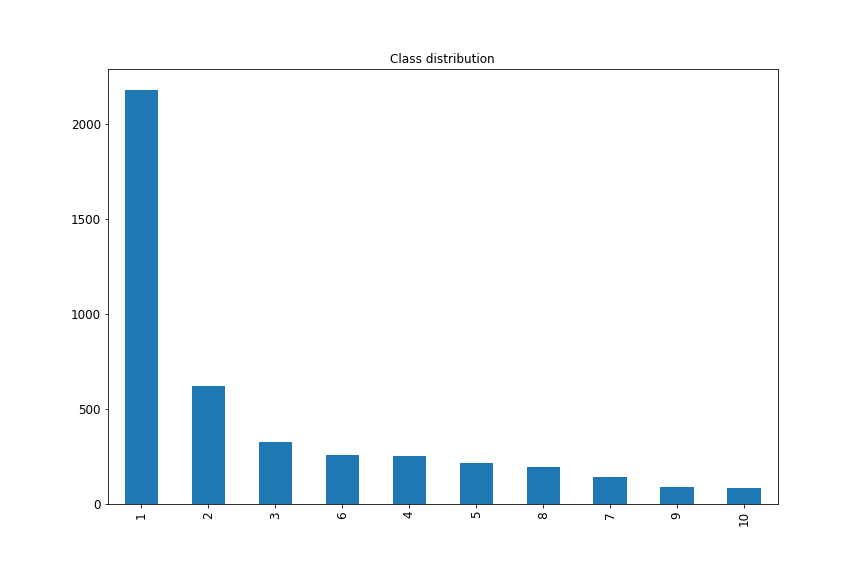
\includegraphics[height = 6cm]{classdistribution.png}
% where an .eps filename suffix will be assumed under latex, 
% and a .pdf suffix will be assumed for pdflatex; or what has been declared
% via \DeclareGraphicsExtensions.
\caption{Histogram showing class distribution}
\label{fig_sim1}
\end{figure}

\subsection{Descriptive statistics}

%The data

Figure 2 shows the descriptive statistics of the data. The horizontal axis contains all of the predictors, with their mean, min, max and quantiles values are shown by the vertical axis. We can see there is some outliers in the first 50 predictors of the dataset

\begin{figure}[!t]
	\centering
	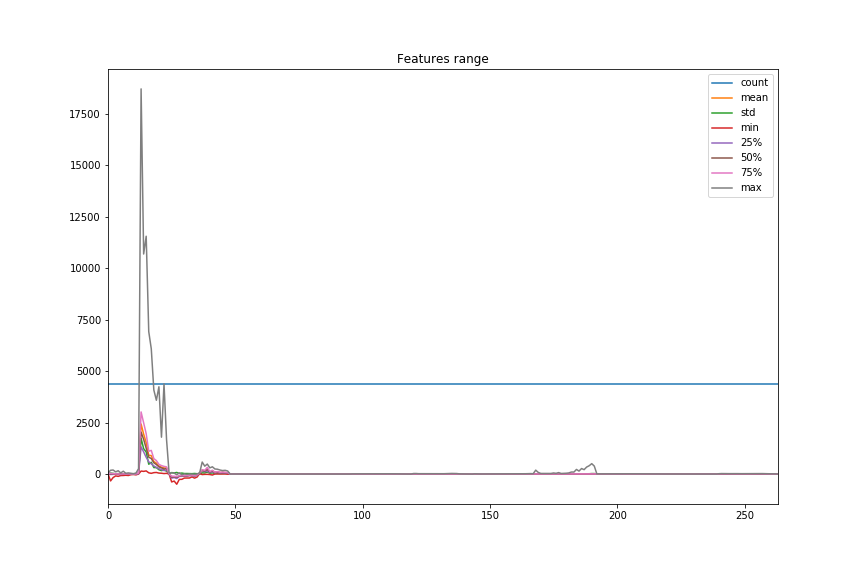
\includegraphics[height = 6cm]{featuresrange.png}
	% where an .eps filename suffix will be assumed under latex, 
	% and a .pdf suffix will be assumed for pdflatex; or what has been declared
	% via \DeclareGraphicsExtensions.
	\caption{Descriptive statistics of the data}
	\label{fig_sim2}
\end{figure}

Figure 3 shows the visualization of the data by the first three orthogonal components that explain the maximum amount of variance. It can be seen that the data seems to be clustered due to the effect of the outliers

\begin{figure}[!t]
	\centering
	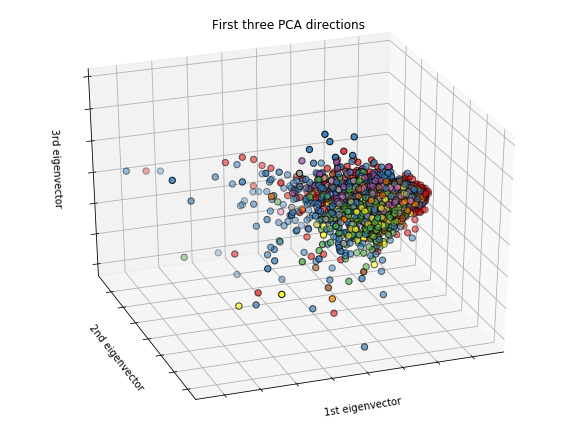
\includegraphics[height = 6cm]{pca.png}
	% where an .eps filename suffix will be assumed under latex, 
	% and a .pdf suffix will be assumed for pdflatex; or what has been declared
	% via \DeclareGraphicsExtensions.
	\caption{Visualization of the data}
	\label{fig_sim3}
\end{figure}

\noindent 
\section{Methods and experiments}
\subsection{Data preprocessing}
Standardization of datasets is a common requirement for many machine learning estimators implemented in scikit-learn; they might behave badly if the individual features do not more or less look like standard normally distributed data: Gaussian with zero mean and unit variance. If a feature has a variance that is orders of magnitude larger than others, it might dominate the objective function and make the estimator unable to learn from other features correctly as expected.
In practice we often ignore the shape of the distribution and just transform the data to center it by removing the mean value of each feature, then scale it by dividing non-constant features by their standard deviation.

As mentioned before, our data contains many outliers (some predictors has over 25\% data points as outliers). Scaling using the mean and variance of the data like above mentioned is likely to not work very well because outliers can often influence the sample mean / variance in a negative way. Therefore I use RobustScaler (sklearn.preprocessing.RobustScaler) to transform our dataset, using statistics that are robust to outliers, i.e. the median and the interquantile range. 
To be specific, this Scaler removes the median and scales the data according to the Interquartile Range - the range between the 1st quartile (25th quantile) and the 3rd quartile (75th quantile). Centering and scaling happen independently on each feature (or each sample, depending on the axis argument) by computing the relevant statistics on the samples in the training set.

%The effect of this scaler on the data can be seen from this figure 
%!!! Figure visualization data after scaling

In my experience, scaling the dataset often improve the performance of ensemble classifiers with trees as base estimators (using boosting or bagging technique)

\subsection{Ensemble model and Gradient boosting:}

I decide to choose boosting as the main method for this problem because boosting is one of the most powerful learning idea introduced in the last twenty years. \cite[chap 10, p338]{elem2} 

The main idea of boosting is based on ensemble learning. In an ensemble mode, a committee of trees (weak learners or base learners) are trained and developed. A single tree model will classify the data points into different leaves, with the score associated with each of the leaves. The final ensemble model is made by combining the prediction of all the base learners, thus become more powerful than a single model. Ensemble learning can be broken down into two tasks: developing a population of base learners from the training data, and then combining them to produce the final prediction.

A boosting model is characterized by how the weak learners are developed and combined: the weak learners evolve over time at each boosting step by additive training (sequentially apply the weak classification algorithm to repeatedly modified versions of the data). \begin{itemize}
\item Initially,  each training observations are given an equal weight $w_i$
and the classifiers (tree learners) is trained on the data in the usual manner
\item For each successive iteration, the observation weights are individually modified so that misclassified data receive more influence. Each successive classifier is thereby forced to concentrate on those training observations that are missed by previous ones in the sequence. The scores are also calculated for each classifier so that we have the contribution of each classifier in the final model
\item Finally, each of the base classifier casts a weighted vote in the final ensemble model to get the final prediction.
\end{itemize}

\subsubsection{numerical optimization via gradient boosting}

\subsection{XGBoost models }
Xgboost (https://github.com/dmlc/xgboost) is chosen because of its high performance in many data science problems in a fast and accurate way.

According to its introduction, Xgboost is an optimized distributed gradient boosting library designed to be highly efficient, flexible and portable. XGboost is still based on gradient boosting framework but it use a more regularized model formalization to control over-fitting, which gives it better performance. It also utilized computational resources better for boosted tree algorithm


A xgboost model has multiple parameters (around 20 to 30) that need to be selected carefully in order to get the best performance while also regularize the overfitting.  

Choose the right size for each tree

Regularlization

To control overfitting, we need to control the parameters "max\_depth", min\_child\_weight and gamma. We can also add noise to the model by control the parameters "subsample" and "colsample\_bytree
"
The problem of unbalanced dataset can be addressed by setting weight for each data point when training the xgboost model
\subsection{ Evaluation: stratified K-fold}
 Scoring accury and log loss
\subsection{Tuning hyperparameters - Bayesian optimization vs Randomsearch}
\subsubsection{Randomsearch}
\subsubsection{Bayesian optimization}


Traditionally, hyperparameter tuning are done by grid search. However, it takes a lot of time to cover a wide range of parameters. Therefore we use Bayesian optimization (https://github.com/fmfn/BayesianOptimization)  

This is a constrained global optimization package built upon bayesian inference and gaussian process, that attempts to find the maximum value of an unknown function in as few iterations as possible. This technique is particularly suited for optimization of high cost functions, situations where the balance between exploration and exploitation is important.  
\subsection{Experiments}


\section{Results}
\subsection{performance measures}
\subsection{performance on Kaggle}
%Confusion matrix

After carrying out the bayesian optimization, we get the result of the best parameters here:
\begin{minted}[%
breaklines,
mathescape,
linenos,
numbersep=5pt,
frame=single,
numbersep=5pt,
xleftmargin=0pt,
]{python}
objective = 'reg:logistic',
learning_rate= 0.1, 
n_estimators = 50,
gamma=0.1, 
max_depth = 12,
min_child_weight = 20,
max_delta_step= 50,
subsample = 0.9,
colsample_bytree = 0.7,
reg_lambda = 0.1,
reg_alpha = 0.1,
\end{minted}

Training xgboost with those parameter on the training set, then make prediction on the test set, we get the following score for test set:

* Accuracy: 0.64654 (position 95) - over the benchmark


* Log-loss: 0.17534 (position 58) - over the benchmark
\section{Conclusion}
Xgboost with gradient boosting works really well in this case

Bayesian opt let us to go over 20 runs (40 mins in total) to select the best xgboost model over a wide range of hyperparameter. IF we use gridsearch, it is expected to spend 10 hours to get the same results


%Feature importance

\section{Appendices}
Code for tuning the xgboost with Bayes optimization
\begin{figure*}
	\caption{Source code}
\begin{minted}[%
breaklines,
mathescape,
linenos,
numbersep=5pt,
frame=single,
numbersep=5pt,
xleftmargin=0pt,
]{python}
def xgbcv(learning_rate, n_estimators, gamma, max_depth, min_child_weight, max_delta_step, subsample, colsample_bytree, reg_lambda, reg_alpha):
	xgb_model =  xgb.XGBClassifier(
		objective = 'multi:softmax',
		learning_rate= max(min(learning_rate, 1), 0), 
		n_estimators = int(n_estimators),
		gamma=max(gamma, 0), 
		max_depth = int(max_depth),
		min_child_weight = int(min_child_weight),
		max_delta_step= int(max_delta_step),
		subsample = max(min(subsample, 1), 0),
colsample_bytree = max(min(colsample_bytree, 1), 0),
reg_lambda = max(reg_lambda, 0),
reg_alpha = max(reg_alpha, 0),
random_state=12345)
val = cross_val_score(xgb_model,
train_data, train_labels, scoring='accuracy',
cv=StratifiedKFold(n_splits=5, random_state=12345, shuffle=False)
).mean()
return val
gp_params = {"alpha": 1e-5}
xgbBO = BayesianOptimization(xgbcv,
{'learning_rate': (0.001, 1), 
'n_estimators': (1, 100),
'gamma': (0.001, 100),
'max_depth': (1, 15),
'min_child_weight': (1, 20),
'max_delta_step': (1, 100),
'subsample': (0.3, 1),
'colsample_bytree': (0.001, 1),
'reg_lambda': (0.001, 100),
'reg_alpha': (0.001, 100)}
)
xgbBO.explore({'learning_rate': [0.001, 0.01, 0.1], 
'n_estimators': [10, 20, 50],
'gamma': [0.001, 0.01, 0.1],
'max_depth': [4, 8, 12],
'min_child_weight': [5, 10, 20],
'max_delta_step': [10, 20, 50],
'subsample': [0.1, 0.45, 0.9],
'colsample_bytree': [0.2, 0.5, 0.7],
'reg_lambda': [0.001, 0.01, 0.1],
'reg_alpha': [0.001, 0.01, 0.1]})
xgbBO.maximize(n_iter=40, **gp_params)
print('-' * 53)
print('Final Results')
print('XGB: %f' % xgbBO.res['max']['max_val'])
\end{minted}
\end{figure*}

\begin{thebibliography}{9}
	\bibitem{elem2}
	Trevor Hastie,	Robert Tibshirani,	Jerome Friedman
	\textit{The Elements of Statistical Learning},
	2nd edition,
	2008
	\bibitem{xgb1}
	Tianqi Chen
	\textit{Introduction to Boosted Trees},
	\url{http://xgboost.readthedocs.io/en/latest/model.html}	
	\bibitem{xgb2}
	Tianqi Chen
	\textit{XgBoost Parameters},
	\url{http://xgboost.readthedocs.io/en/latest/parameter.html}	
\end{thebibliography}

% biography section
% 
% If you have an EPS/PDF photo (graphicx package needed) extra braces are
% needed around the contents of the optional argument to biography to prevent
% the LaTeX parser from getting confused when it sees the complicated
% \includegraphics command within an optional argument. (You could create
% your own custom macro containing the \includegraphics command to make things
% simpler here.)
%\begin{IEEEbiography}[{\includegraphics[width=1in,height=1.25in,clip,keepaspectratio]{mshell}}]{Michael Shell}
% or if you just want to reserve a space for a photo:

%\begin{IEEEbiography}{Michael Shell}
%Biography text here.
%\end{IEEEbiography}

%\begin{IEEEbiography}{Zhengyu Peng}
%Biography text here.
%\end{IEEEbiography}

% if you will not have a photo at all:
%\begin{IEEEbiographynophoto}{John Doe}
%Biography text here.
%\end{IEEEbiographynophoto}

% insert where needed to balance the two columns on the last page with
% biographies
%\newpage

%\begin{IEEEbiographynophoto}{Jane Doe}
%Biography text here.
%\end{IEEEbiographynophoto}

% You can push biographies down or up by placing
% a \vfill before or after them. The appropriate
% use of \vfill depends on what kind of text is
% on the last page and whether or not the columns
% are being equalized.

%\vfill

% Can be used to pull up biographies so that the bottom of the last one
% is flush with the other column.
%\enlargethispage{-5in}

% that's all folks

\end{document}
